\chapter{Аналитический раздел}


\section{Анализ предметной области}

Продажи алкоголя в России выросли на 2\% в 2022 году. Это следует из итогового доклада министерства здравоохранения России\cite{minzdrav} за год. Российские виноделы увеличили производство за январь-апрель 2023 года по сравнению с аналогичным периодом прошлого года на 10\%, по данным Минсельхоз РФ\cite{selhoz}. 

В Российской Федерации запрещена доставка алкогольной продукции, к которой относится и вино, пунктом 5 правил продажи товаров дистанционным способом\cite{pravila}. Поэтому в России не нужно реализовывать функционал по доставке вин. После оформления заказов с алкоголем покупатели должны лично приехать в магазин или на склад и забрать товар. 

Интернет магазин должен предоставлять доступ к перечню вин, а также поддерживать возможность добавления и удаления вин в заказе. Покупатели должны иметь возможность для легкого оформления заказа. Бонусные баллы сподвигнут пользователей на последующие покупки и помогут привлечь постоянных клиентов. Также раздел <<любимое>> поможет покупателям отложить вино, чтобы вернуться к нему попозже и купить.


\section{Постановка задачи}

Необходимо разработать приложение винного магазина. Авторизованным пользователям предоставлен доступ к ассортименту вин, 
а также возможность формировать заказы. Пользователь может добавлять и удалять вина из заказа. Заказы могут быть оплачены рублями или полностью баллами. Если заказ оплачен рублями, то клиенту начисляется баллами 10\% от суммы заказа после подтверждения оплаты. Также пользователь может добавлять вина в раздел <<любимое>>. Администратор может добавлять новую позицию вина в каталог, удалять и обновлять уже существующие позиции в каталоге, также администратор подтверждает оплату счета.


\section{Формализация данных}

База данных состоит из таблиц:
\begin{enumerate}[label=\arabic*)]
	\item Таблица вин wine.

 Хранит в себе сведения о винах: название, количество оставшихся бутылок, год, крепость, цену, страну и сорт.
 
	\item Таблица пользователей user.

  Содержит данные пользователей: логин, пароль, ФИО, электронную почту, баллы, права доступа.
  
	\item Таблица заказов order.

Включает в себя владельца заказа, общую стоимость заказа, статус заказа, тип оплаты.

        \item Таблица элементов заказа order\_element.

Содержит сведения об элементе заказа: вине; количестве заказанных бутылок; заказе, к которому принадлежит.
        
        \item Таблица счетов bill.

Хранит в себе сведения о счете: заказ, статус и сумма к оплате.    

        \item Таблица для <<любимых>> вин user\_wine.

        Содержит идентификационный номер пользователя и идентификационный номер вина как внешние ключи.
\end{enumerate}

На рисунке \ref{img:er} представлена ER-диаграмма сущностей проектируемой базы данных в нотации Чена.
% \begin{figure}[H]
% 	\centering
% 	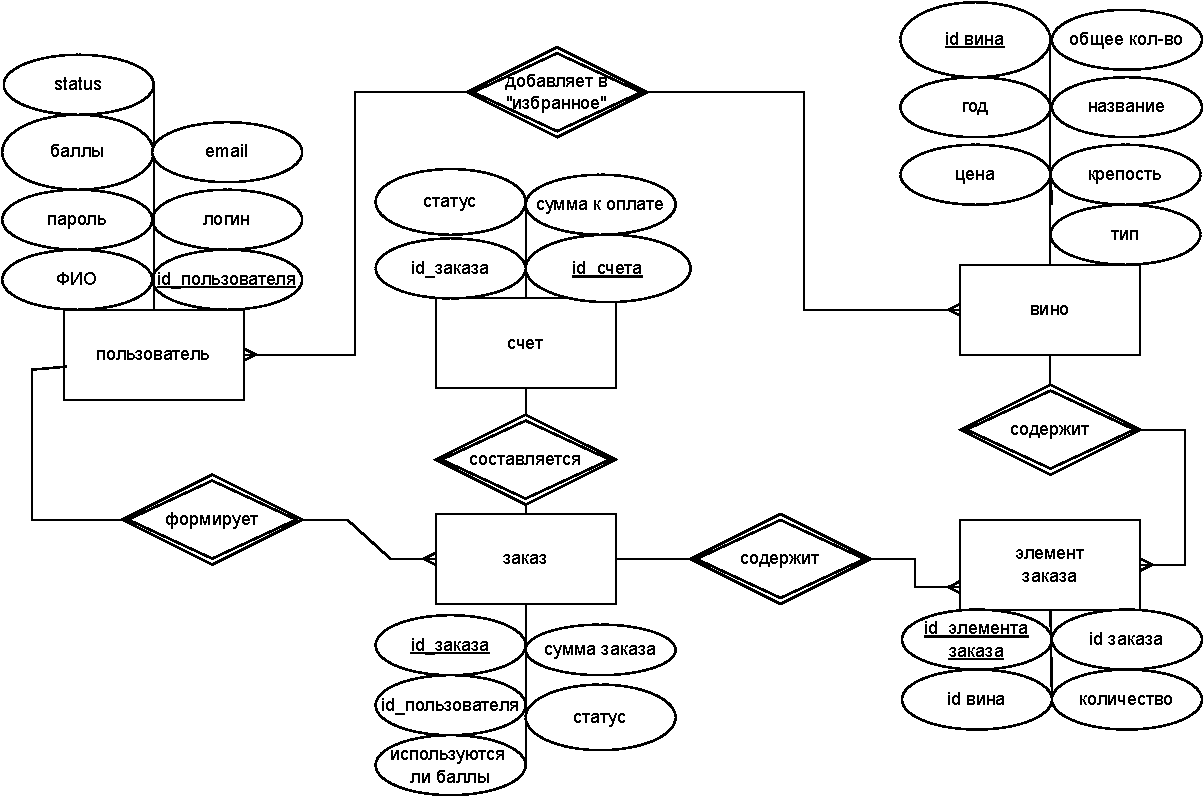
\includegraphics[scale=0.8]{include/er.pdf}
% 	\caption{ER-диаграмма сущностей проектируемой базы данных в нотации Чена}
% 	\label{img:er}
% \end{figure} 

\includeimage
    {er} % Имя файла без расширения (файл должен быть расположен в директории inc/img/)
    {f} % Обтекание (без обтекания)
    {h} % Положение рисунка (см. figure из пакета float)
    {0.75\textwidth} % Ширина рисунка
    {ER-диаграмма сущностей проектируемой базы данных в нотации Чена} % Подпись рисунка
\newpage

\section{Типы пользователей}

Выделено три вида пользователей: незарегистрированный пользователь, зарегистрированный пользователь и администратор. Для каждого типа пользователей предусмотрен
свой набор возможностей. 

 На рисунке \ref{img:usecases} представлена Use-Case диаграмма использования приложения.

\includeimage
    {usecases} % Имя файла без расширения (файл должен быть расположен в директории inc/img/)
    {f} % Обтекание (без обтекания)
    {h} % Положение рисунка (см. figure из пакета float)
    {0.8\textwidth} % Ширина рисунка
    {Use-Case диаграмма использования приложения} % Подпись рисунка
\newpage    
% \begin{figure}[H]
% 	\centering
% 	\includegraphics[scale=0.8]{include/usecase.pdf}
% 	\caption{Use-Case диаграмма использования приложения}
% 	\label{img:use-case}
% \end{figure} 


\section{Общие сведения о БД и СУБД}
База данных (БД) — это совокупность данных, хранимых в упорядоченной форме, с целью обеспечения доступа к этим данным и их использования
каким-либо организационными или прикладными процессам \cite{bd}.

Система управления базами данных (СУБД) – это совокупность программ
и языковых средств, предназначенных для управления данными в базе данных,
ведения базы данных и обеспечения взаимодействия её с прикладными программами \cite{subd}.

\section{Описание существующих моделей данных}
Базы данных разделяют на два основных типа: реляционные и нереляционные. Последние делятся ещё на два: сетевые и иерархические. Хоть и существует очень большое число видов баз данных, но их всех можно классифицировать по модели данных, которая определяет логическую
структуру БД:
\begin{enumerate}
    \item сетевая модель --- используют структуру в виде графа.;
    \item иерархическая модель ---  использует структуру данных в виде деревьев;
    \item реляционная модель --- использует табличное представление данных.
\end{enumerate}


\subsection{Сетевая модель}

Сетевая БД состоит из набора экземпляров определенного типа записи и набора экземпляров определенного типа связей
между этими записями \cite{setevy}. Данную модель можно представить в виде сети, состоящей из узлов, которые могут иметь несколько связей. Она облегчает доступ к данным, так как вместо указания адреса нужной ячейки, данные можно получить, сделав запрос на поиск дочернего объекта.

Сетевая модель имеет свои преимущества и недостатки. Основным преимуществом является гибкость и эффективность поиска информации. Однако главным недостаток остается
невозможность изменить структуру после ввода данных. Также, в связи с трудностью моделирования сложных структур данных, могут возникать сложности в управлении и обслуживании базы данных.

\subsection{Иерархическая модель}

В иерархической модели данных используется представление базы данных в
виде древовидной структуры, где между объектами существуют связи предок-потомок, при этом объект-предок может иметь неограниченное количество потомков, тогда как у объекта-потомка обязательно будет только один предок \cite{ierarch}. 

Основным преимуществом иерархической модели является высокая скорость доступа к данным. Это происходит за счет прямого доступа к узлам в древовидной структуре иерархии данных. Кроме того, данная модель данных является простой в использовании и понимании, что позволяет легко создавать и изменять базы данных.

Главным недостатком иерархической модели является ограничение в возможностях представления сложных связей между данными. Это ограничивает варианты использования.


\subsection{Реляционная модель}
Реляционная модель данных является совокупностью данных и основана на использовании таблиц, которые связаны между собой посредством отношений \cite{relyac}. Каждая таблица состоит из строк и столбцов, каждый столбец имеет имя и определенный тип данных. На
пересечении строк и столбцов находятся конкретные значения.

Основным преимуществом реляционной модели является легкость ее использования и гибкость в изменении данных. Она позволяет быстро создавать и изменять таблицы и связи. 

Недостатком реляционной модели является ограничение в представлении сложных структур данных. Кроме того, она может быть менее эффективной в случаях, когда требуется быстрый доступ к большим объемам данных.

В настоящее время реляционная модель является наиболее широко используемой
формой представления данных в различных областях.

Для разработки была выбрана реляционная модель базы данных,
будет использоваться PostgreSQL, как один из наиболее популярных реляционных СУБД и так как имеется опыт разработки на нем.


\section{Анализ существующих решений}

Из числа ранее существующих <<конкурентов>>, было выделено 3 решения. Сравнение существующих решений проводилось по следующим критериям:
\begin{enumerate}[label=\arabic*)]
\itemвозможность покупки за баллы;
\itemориентированность на продажу вина;
\itemподдержка русского языка.
\end{enumerate}

В таблице \ref{table:change} приведено сравнение других решений по данным критериям.
\newpage
\begin{table}[H]
	\begin{center}
		\caption{Сравнение существующих решений}
		\label{table:change}
  \begin{tabular}{ | p{4cm} | p{3cm} | p{4cm} | p{3cm}|}
    \hline
    {Название}&{возможность покупки за баллы}&{ориентированность на продажу вина}&{поддержка русского языка}\\ \hline
   
    {Красное\&Белое\cite{cb}}&{нет}&{нет}&{есть}
			\\ \hline

    {ВИНЛАБ\cite{winlab}}&{есть}&{нет}&{есть}
			\\ \hline

   {wine.com\cite{wine}}&{нет}&{есть}&{нет}
			\\ \hline
  \end{tabular}
\end{center}
\end{table}

Представленные решения не удовлетворяют всем требованиям: некоторые цифровые магазины не позволяют совершать покупки за баллы, многие продают не только вина, но и другие товары, а некоторые попросту не поддерживают русский язык, что приносит неудобства покупателям из России.

